\subsection{McCulloch-Pitts-Neuron}

\begin{frame}
\frametitle{Zusammenhang - Biologisches Neuron}

\begin{figure}
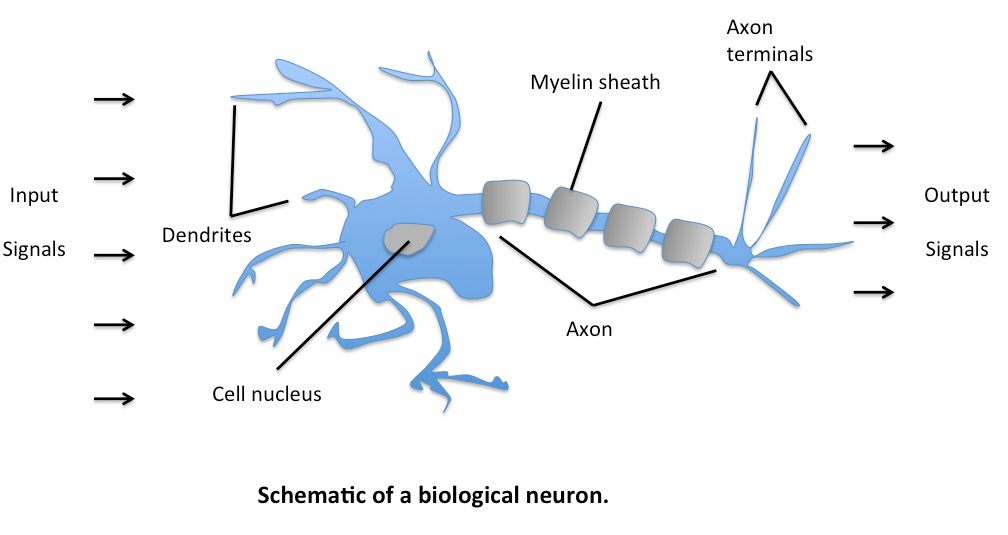
\includegraphics[width=\linewidth]{./geschichtliches/mcCullochPittsNeuron/img/bioNeuron_alpha}
\end{figure}

\note[item]{\emph{Dendriten}: Nehmen Infos auf
\begin{itemize}
  \item besizten Rezeptoren und Signale anderer Dendriten aufzunehmen
\end{itemize}}

\note[item]{Signale: bewirken elektrische Veränderungen
\begin{itemize}
  \item werden vom Zellkern (Soma) interpretiert / verarbeitet
  \item Zellkern sammelt Infos, speichert diese im Axonhügel
\end{itemize}}

\note[item]{Ursprung vom Axon / Neuriten}
\note[item]{Wenn Signal stark genug: an Axon weitergeleitet
\begin{itemize}
  \item auch als \emph{Aktionspotential bezeichnet}
  \item Signal am Ende über Axonterminale per Neurotransmitter mit nächste Dendriten verbunden
\end{itemize}}

\end{frame}


\begin{frame}
\frametitle{McCulloch-Pitts-Neuron}

\begin{columns}

\column{0.5\textwidth}
\begin{itemize}
	\item Modell soll Funktionalität des biologischen Neurons imitieren
	\item Klassifizierungsproblem als grundlegende Problemstellung
	\item Lineare Entscheidungsfunktion zur binären Klassifizierung verwendet
\end{itemize}


\column{0.5\textwidth}
\begin{figure}
	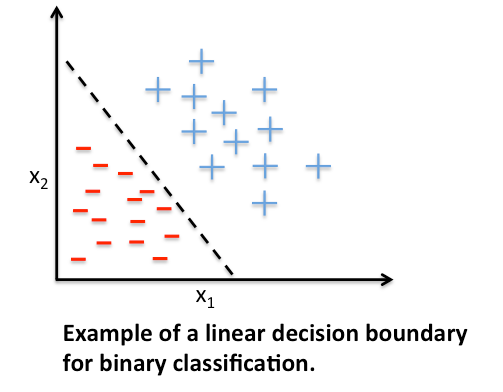
\includegraphics[width=\linewidth]{./geschichtliches/mcCullochPittsNeuron/img/bnKlassifizierung_alpha}
\end{figure}

\end{columns}


\note[item]{1943: Warren McCulloch \& Walter Pitts}
\note[item]{soll biologisches Neuron imitieren}
\note[item]{Klassifizierungsproblem: anhand vom geg. Merkmalsvektor entscheiden ob Objekt X in Klasse K liegt}
\note[item]{hier lediglich binäre Klassifikation
\begin{itemize}
    \item Unterscheidung nur zwischen zwei Klassen
    \item Sonderfall dieses Modells: nur boolesche Eingabewerte
\end{itemize}}
\note[item]{muss mittels linearer Entscheidungsfunktion definierbar sein}

\end{frame}


\begin{frame}
\frametitle{Aufbau und Funktionsweise}
\begin{figure}
	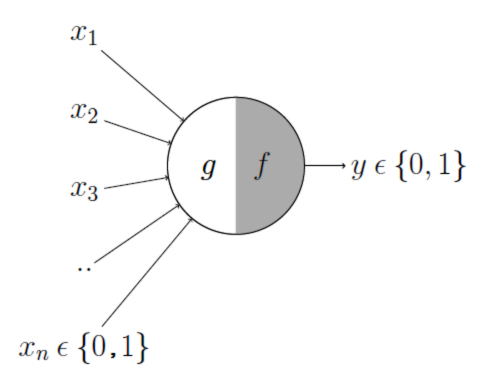
\includegraphics[width=.5\linewidth]{./geschichtliches/mcCullochPittsNeuron/img/aufbau_alpha}
\end{figure}

\hrule

\begin{columns}

\column{0.4\textwidth}
\begin{align*}
g(x_1, x_2, \dots , x_n) = g(x) = \sum_{i=1}^n x_i
\end{align*}

\column{0.4\textwidth}
\begin{align*} \label{eq:aktFkt2}
f(g(x)) =\begin{cases}
	1 & \mbox{if } g(x) \geq \theta \\
    0 & \mbox{if } g(x) < \theta
  \end{cases}
\end{align*}
\end{columns}

\note[item]{beliebig viele Eigabewerte
\begin{itemize}
    \item müssen boolescher Natur sein
\end{itemize}}

\note[item]{Arbeitsschritte:
\begin{itemize}
    \item Alle Werte aufaddiert (Fkt. \emph{g})
    \item Fkt. \emph{f} prüft ob Schwellwert überschritten
\end{itemize}}

\note[item]{Es folgt: Logik Gattter mit Modell dargestellt}

\end{frame}


\begin{frame}
\frametitle{Notation AND-Gatter}

\begin{figure}
	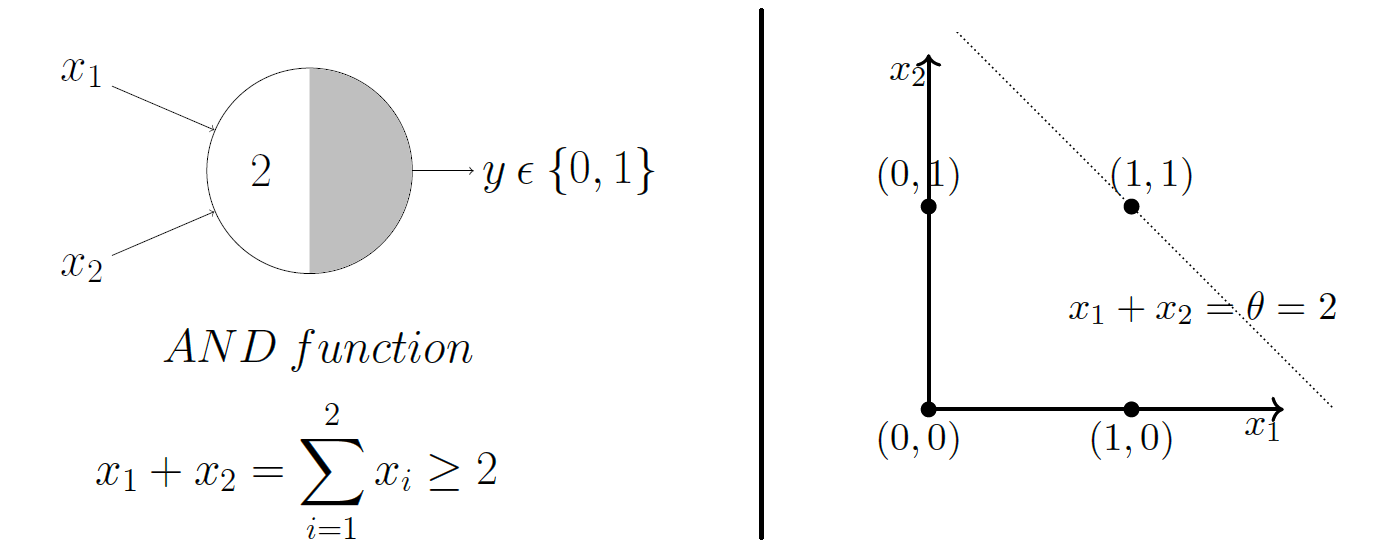
\includegraphics[width=\linewidth]{./geschichtliches/mcCullochPittsNeuron/img/mpn_and_alpha}
\end{figure}

\note[item]{Anhand von Grafik erläutern}
\note[item]{Schwellwert auf der linken Seite notiert}

\end{frame}


\begin{frame}
\frametitle{Notation OR-Gatter}

\begin{figure}
	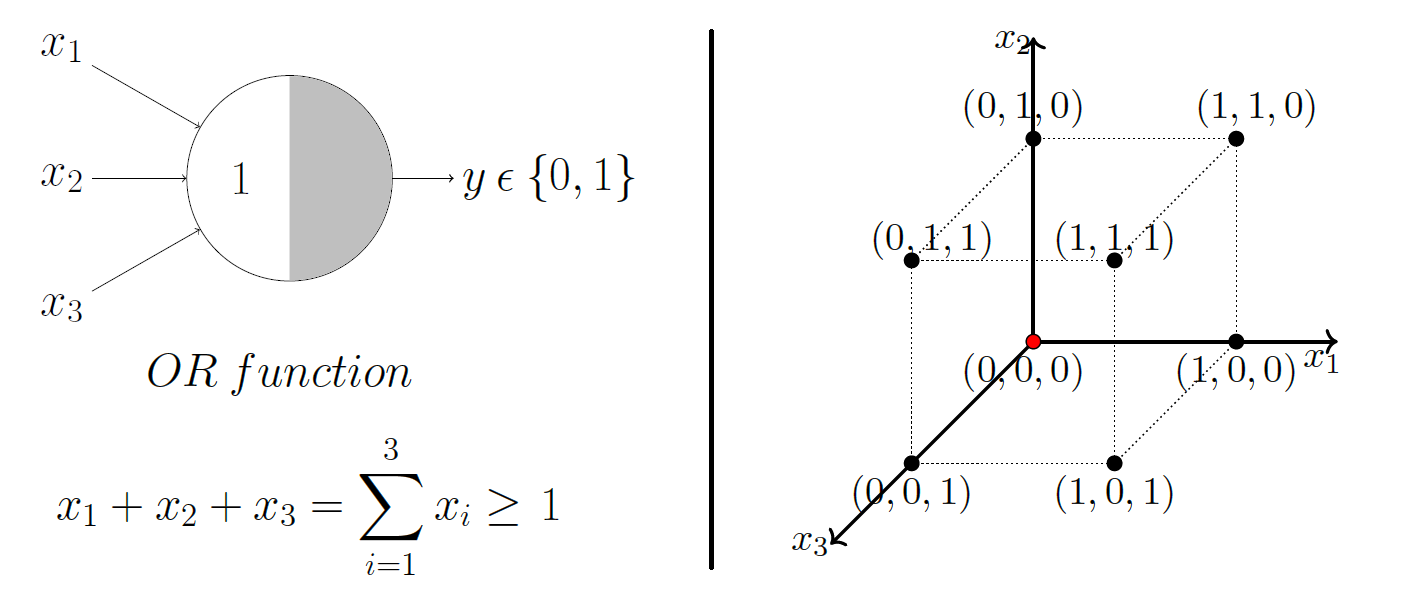
\includegraphics[width=\linewidth]{./geschichtliches/mcCullochPittsNeuron/img/mpn_or_alpha}
\end{figure}

\note[item]{Anhand von Grafik erläutern, auch im 3d - Raum möglich}

\end{frame}


\begin{frame}
\frametitle{Nachteile}

\begin{itemize}
\item Keine kontinuierlichen Eingabewerte (nur boolesche Werte)
\item Schwelle muss manuell gesetzt werden, keine automatische Aktualisierung vorgesehen
\item Keine Priorisierungsmöglichkeit der Eingabewerte möglich
\item Funktionen müssen durch lineare Entscheidungsfunktion getrennt werden können
\end{itemize}

\begin{columns}
\column{.4\textwidth}
\begin{figure}
	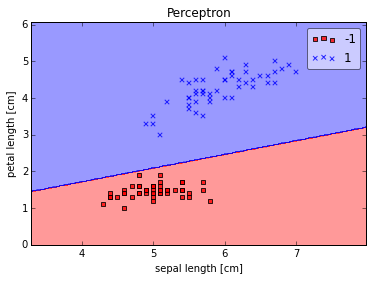
\includegraphics[width=\linewidth]{./geschichtliches/mcCullochPittsNeuron/img/perceptron_klassifizierung1}
\end{figure}

\column{.4\textwidth}
\begin{figure}
	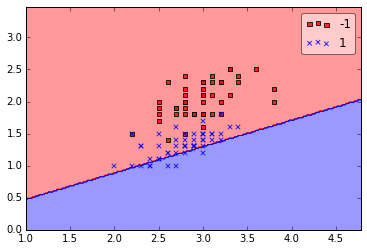
\includegraphics[width=\linewidth]{./geschichtliches/mcCullochPittsNeuron/img/perceptron_klassifizierung2}
\end{figure}


\end{columns}

\note[item]{keine kontinuierlichen Eingabewerte
\begin{itemize}
    \item nur boolesche Werte
    \item Schwierig für komplexe Anwendungen 
    \item siehe Bilderkennung - Farbwerte
\end{itemize}}

\note[item]{Schwelle muss manuelle gesetzt werden
\begin{itemize}
    \item Sprich kein Lernalgorithmus vorhanden
\end{itemize}}

\note[item]{Keine Priorisierungsmöglichkeiten
\begin{itemize}
    \item siehe Gewichtete Eingaben
\end{itemize}}

\note[item]{Funktionen durch lineare Entscheidungsfunktion getrennt
\begin{itemize}
    \item schwierig bei überlappenden Cluster
    \item keine Polynome wie bei späteren Entwicklungen möglich
\end{itemize}}

\note[item]{auch gedeckelte Fkt. wie XOR können nicht dargestellt werden
\begin{itemize}
    \item Schwelle muss genau getroffen werden
\end{itemize}}

\end{frame}
